\documentclass{beamer}

\usetheme{Montpellier}
%\usetheme{CambridgeUS}


\usepackage[OT1]{fontenc}
\usepackage[utf8x]{inputenc}


%\usepackage[T1]{fontenc}
%\usepackage[latin9]{inputenc}
\usepackage[german]{babel}
\usepackage{booktabs,bm, color, enumerate, hyperref, pgf, url, soul, tikz}
\usepackage{amssymb, amsmath}
\usepackage{graphicx}
\newcommand*{\Scale}[2][4]{\scalebox{#1}{$#2$}}%
\newcommand*{\Resize}[2]{\resizebox{#1}{!}{$#2$}}%

%\usepackage{hyperref}

\usepackage{appendixnumberbeamer}


\bibliographystyle{apalike}



%\input{abbreviations}



\setbeamertemplate{blocks}[rounded][shadow=true]
%\usepackage{appendixnumberbeamer}



%\subject{2015}




\title{Advanced Regression: 3c Prediction accuracy and cross-validation}



\author{Garyfallos Konstantinoudis}
\institute{Epidemiology and Biostatistics, Imperial College London}



\date{7th March 2023}


\setlength{\unitlength}{0.9cm}
\linethickness{1.1pt}








\begin{document}


\frame{
\titlepage
}



\frame{
\tableofcontents
}



%\section{Prediction and Overfitting}
%\section{Cross-validation}
%\subsection{Cross-validation for parameter}
%\subsection{Cross-validation to evaluate prediction performance}
%\section{Cross-validation in practice}



\section{Cross-validation (CV)}



\frame{
\frametitle{CV as a re-sampling technique} 

Tools that involve repeatedly drawing samples from a training set and refitting a model on each sample.
In each draw we obtain more information about the fitted model.


\begin{block}{Aims}{
\begin{enumerate}
\item  To evaluate prediction rules and compare different models with respect to their predictive performance.
\item  To fix open parameters and set model complexity, e.g. $\lambda$ the regularization parameter in regularized regression. 
\end{enumerate}
}
\end{block}


}

\frame{
\frametitle{CV approaches} 

\begin{enumerate}
\item Exhaustive cross-validation
\begin{itemize}
\item Leave-one-out cross-validation
\item Leave-$p$-out cross-validation
\end{itemize}
\item Non-exhaustive cross-validation
\begin{itemize}
\item $k$-fold cross-validation
\item Repeated random sub-sampling validation
\end{itemize}
\end{enumerate}

}


\subsection{Exhaustive cross-validation}


\frame{
\frametitle{Leave-one-out cross-validation (LOOCV)} 


\begin{itemize}
\item Split the data containing $n$ observations into
\begin{enumerate}
\item Training data of size $n-1$
\item Test data of size $1$
\end{enumerate}
\item In each split, we leave out \textbf{one} observation.
\item We fit the prediction rule $\hat{f}(x)$ on the training data without observation $i$.
\item We evaluate the $MSE_i$ of $\hat{f}(x_i)$ on the single observation $i$.
\item Repeat $n$-times for $i \in 1,...,n$.
\item Overall mean CV test error is defined as
\begin{equation}
CV_{\{n\}} = \frac{1}{n} \sum_{i=1}^n MSE_i \nonumber
\end{equation} 
\end{itemize}

}

\frame{
\frametitle{Leave-one-out cross-validation (LOOCV)} 


\centering 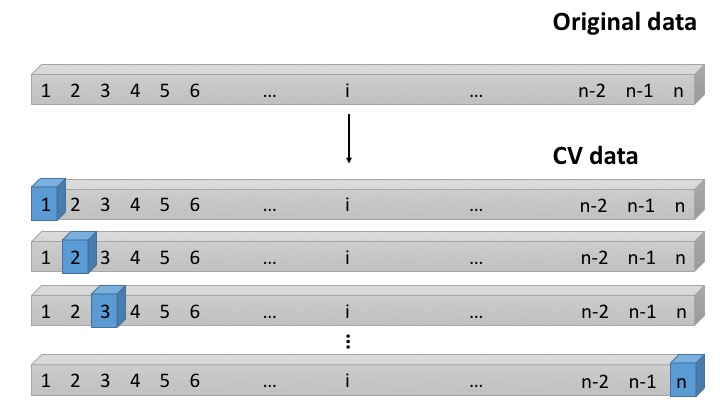
\includegraphics[scale=0.44]{E:/Postdoc Imperial/Lectures/2023_AdvancedRegression/AdvancedRegression2022-2023/lectures/graphs/cv-loo}



}


\frame{
\frametitle{Leave-$p$-out cross-validation (LOOCV)} 


\begin{itemize}
\item Split the data containing $n$ observations into
\begin{enumerate}
\item Training data of size $n-p$
\item Test data of size $p$
\end{enumerate}
\item In each split, we leave out \textbf{$p$} observations.
\item We fit the prediction rule $\hat{f}(x)$ on the training data without the $p$ observations.
\item We evaluate the $MSE_i$ of $\hat{f}(x_i)$ on the test data $i \in p$.
\item Repeat for all possible combinations $comb = \binom{n}{p}$ of how to select $p$ elements from a set of $n$.
\item Overall mean CV test error is defined as
\begin{equation}
CV_{\{comb\}} = \frac{1}{comb} \sum_{i=1}^{comb} MSE_i \nonumber
\end{equation} 
\end{itemize}

}


\subsection{Non-exhaustive cross-validation}


\frame{
\frametitle{$k$-fold cross-validation} 


\begin{itemize}
\item With k-fold CV, we divide the data set into $k$ different subsets, each of the same length.
\item Recommended are $k=5$ or $k=10$.
\item We fit the prediction rule $\hat{f}(x)$ on the training data including $k-1$ subsets.
\item We evaluate the $MSE_g$ of $\hat{f}(x_g)$ on all observations $g$ in subset $k$.
\item Repeat $k$-times for $g \in 1,...,k$.
\item Overall CV test error rate is defined as
\begin{equation}
CV_{k-fold} = \frac{1}{k} \sum_{g=1}^k MSE_g \nonumber
\end{equation} 
\end{itemize}


}


\frame{
\frametitle{$k$-fold cross-validation} 


\centering 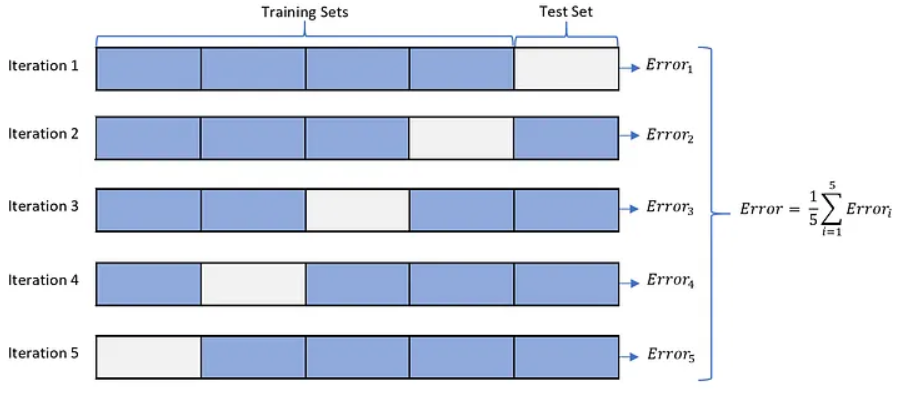
\includegraphics[scale=0.44]{E:/Postdoc Imperial/Lectures/2023_AdvancedRegression/AdvancedRegression2022-2023/lectures/graphs/cvk.png}

}


\frame{
\frametitle{Repeated random sub-sampling validation} 

\begin{itemize}
\item Also known as Monte Carlo CV.
\item Randomly splits the dataset into training and test data. 
\item Advantage: The proportion of the training/test split is not dependent on the folds.
\item No guarantee that the samples are evenly distributed among training and test data, e.g. some samples might only ever be in the training data and never used to test the prediction.
\end{itemize}

}

\frame{
	\frametitle{MC cross validation} 
	
	
	\centering 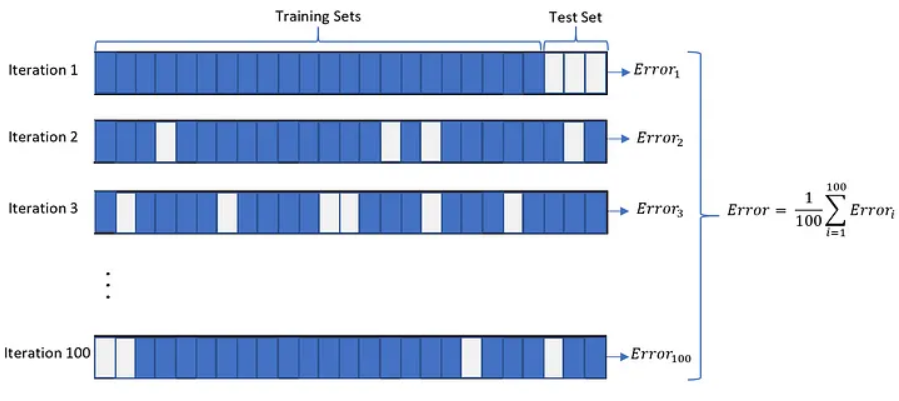
\includegraphics[scale=0.44]{E:/Postdoc Imperial/Lectures/2023_AdvancedRegression/AdvancedRegression2022-2023/lectures/graphs/cvmc.png}
	
}



\frame{
\frametitle{Comparison LOOCV and $k$-fold CV} 

\begin{itemize}
\item LOOCV is a special case of $k$-fold CV, when $n=k$.
\item LOOCV has less bias than $k$-fold CV.
\item LOOCV has higher variance than $k$-fold CV.
\item LOOCV is deterministic, while $k$-fold CV depends on the random draw of the folds.
\item LOOCV ($n$ iterations) is more computationally intensive than $k$-fold CV ($k$ iterations).
\item L-$p$-OCV ($\binom{n}{p}$ iterations) is computationally infeasible for medium sample size.
For example $p=10$ out of $n$ has over $e+13$ possible combinations (\texttt{R: choose(100,10)}).
\end{itemize}

}





\section{Cross-validation to evaluate prediction performance}

\frame{
	\frametitle{Cross-validation to evaluate prediction rules} 
	
	We can use CV: 
	\begin{itemize}
		\item To evaluate the prediction performance of different methods, e.g. Ridge regression against Elastic Net.
		\item To compare different models with different predictors (not necessarily nested) and decide which model has the better prediction performance.
		\item To examine how well a prediction rule generalises to the population (given that our data was representative). 
	\end{itemize}
	
	\begin{block}{CV is build to evaluate prediction performance.}{
			It does not help us to understand how the individual components of a model work.
		}
	\end{block}
	
}





\subsection{Cross-validation in R: \texttt{crossval}}

\frame{
	\frametitle{Cross-validation in R: \texttt{crossval}} 
	
	Example: Prediction of Diabetes disease progression
	\begin{itemize}
		\item Does the prediction improve when we add blood lipid measurements to our model?
	\end{itemize}
	
	\vspace{0.4cm}
	
	\includegraphics[scale=0.4]{E:/Postdoc Imperial/Lectures/2023_AdvancedRegression/AdvancedRegression2022-2023/lectures/graphs/diabetes-mse1}
	
	
}


\frame{
	\frametitle{Cross-validation in R: \texttt{crossval}} 
	
	\begin{enumerate}
		\item Write a prediction function.
	\end{enumerate}
	
	\centering \includegraphics[scale=0.46]{E:/Postdoc Imperial/Lectures/2023_AdvancedRegression/AdvancedRegression2022-2023/lectures/graphs/diabetes-mse2}
	
	
}


\frame{
	\frametitle{Cross-validation in R: \texttt{crossval}} 
	
	\begin{enumerate}
		\item[2.] Load the \texttt{crossval} package and perform the CV for model \texttt{x} (including blood lipids) and \texttt{x1} (excluding blood lipids).
		\includegraphics[scale=0.42]{E:/Postdoc Imperial/Lectures/2023_AdvancedRegression/AdvancedRegression2022-2023/lectures/graphs/diabetes-mse3}
		\item[3.] Evaluate the CV test error rate for  \texttt{x} and  \texttt{x1}.
		\includegraphics[scale=0.44]{E:/Postdoc Imperial/Lectures/2023_AdvancedRegression/AdvancedRegression2022-2023/lectures/graphs/diabetes-mse4}
		\item[4.] Model  \texttt{x} has a lower CV test error than \texttt{x1}.
		$\rightarrow$ Lipid measurements improve the prediction of disease progression.
	\end{enumerate}
	
	
}





\section{Cross-validation to fix open parameters}

\frame{
	\frametitle{Cross-validation to fix open parameters} 
	
	\begin{itemize}
		\item Many algorithms have open parameters.
		\item Example: Penalisation parameter $\lambda$ in regularized regression
		\begin{equation}
		\underset{\alpha, \beta}{argmin} =  RSS(\alpha,\beta) +  \lambda f(\beta) \nonumber
		\end{equation}
		\item It is not recommended to fix those parameter arbitrary since we might not understand what the consequences are.
		\item Cross-validation can be used to fix these parameters with respect to the prediction performance of a model.
		\item Again, cross-validation tunes the parameter to optimise prediction performance, this is not to help us understand a model.
	\end{itemize}
	
	
}



\frame{
	\frametitle{Cross-validation to fix open parameters} 
	
	
	\begin{itemize}
		\item Both the MSE in LOOCV and the MSE in $k$-fold CV are random variables.
		\item The mean CV test error is an estimate for the expected CV test error.
		\begin{itemize}
			\item[$\diamond$] LOOCV
			\begin{equation}
			CV_{\{n\}} = \frac{1}{n} \sum_{i=1}^n MSE_i \nonumber
			\end{equation}
			\item[$\diamond$] $k$-fold CV
			\begin{equation}
			CV_{k-fold} = \frac{1}{k} \sum_{g=1}^k MSE_g \nonumber
			\end{equation} 
		\end{itemize}
		\item Each  mean CV test error has a variance and a standard error.
	\end{itemize}
	
	
	\begin{block}{Occam's razor}{
			Select the largest value of $\lambda$ (smallest model) such that error is within 1 standard error of the minimum CV error.
		}
	\end{block}
	
}


\frame{
	\frametitle{Cross-validation to fix open parameters} 
	
	
	\centering \includegraphics[scale=0.44]{E:/Postdoc Imperial/Lectures/2023_AdvancedRegression/AdvancedRegression2022-2023/lectures/graphs/MSE-1se}
	
	
}






\section{Cross-validation in R: \texttt{cv.glmnet}}

\frame{
	\frametitle{Cross-validation in R: \texttt{cv.glmnet}} 
	
	\begin{itemize}
		\item The R package \texttt{glmnet} has its own inbuilt function to perform CV: \texttt{cv.glmnet}.
		\item When computing a glmnet object without pre-specified $\lambda$ \texttt{glmnet} computes the model over a grid of lambdas and returns a matrix of regression coefficients.
	\end{itemize}
	
	\centering \includegraphics[scale=0.46]{E:/Postdoc Imperial/Lectures/2023_AdvancedRegression/AdvancedRegression2022-2023/lectures/graphs/glmnet-cv1}
	
	
}

\frame{
	\frametitle{Cross-validation in R: \texttt{cv.glmnet}} 
	
	\begin{itemize}
		\item \texttt{glmnet} defines the optimal grid of lambda values for you.
	\end{itemize}
	
	\includegraphics[scale=0.33]{E:/Postdoc Imperial/Lectures/2023_AdvancedRegression/AdvancedRegression2022-2023/lectures/graphs/glmnet-cv2}
	
	
}


\frame{
	\frametitle{Cross-validation in R: \texttt{cv.glmnet}} 
	
	\texttt{cv.glmnet} performs the CV and returns two values:
	\begin{enumerate}
		\item $\$$lambda.min: The $\lambda$ with the minimum CV error 
		\item $\$$lambda.1se: The $\lambda$ within 1 standard error of the minimum CV error, that provides the sparsest model 
	\end{enumerate}
	
	\vspace{0.4cm}
	
	\includegraphics[scale=0.35]{E:/Postdoc Imperial/Lectures/2023_AdvancedRegression/AdvancedRegression2022-2023/lectures/graphs/glmnet-cv3}
	
	
}


\frame{
	\frametitle{Cross-validation in R: \texttt{cv.glmnet}} 
	
	\begin{itemize}
		\item Note: CV is not deterministic. 
		\item When you repeat the CV, you can see different CV mean errors and the respective optimal lambdas.
	\end{itemize}
	
	\vspace{0.2cm}
	
	\includegraphics[scale=0.35]{E:/Postdoc Imperial/Lectures/2023_AdvancedRegression/AdvancedRegression2022-2023/lectures/graphs/glmnet-cv4}
	
	
}


\frame{
	\frametitle{Cross-validation in R: \texttt{cv.glmnet}} 
	
	\begin{itemize}
		\item In order to synchronise the random number generator in \texttt{R} and reproduce your results use
		\texttt{set.seed()}.
	\end{itemize}
	\vspace{0.2cm}
	
	\includegraphics[scale=0.35]{E:/Postdoc Imperial/Lectures/2023_AdvancedRegression/AdvancedRegression2022-2023/lectures/graphs/glmnet-cv5}
	
	
}


\frame{
	\frametitle{Cross-validation in R: \texttt{cv.glmnet}} 
	
	\begin{itemize}
		\item To extract the lasso model with cross-validated lambda, run first the CV and then extract the model with the specific lambda.
		\vspace{0.2cm}
		\includegraphics[scale=0.3]{E:/Postdoc Imperial/Lectures/2023_AdvancedRegression/AdvancedRegression2022-2023/lectures/graphs/glmnet-cv6}
		\item Shortcut:
		\includegraphics[scale=0.35]{E:/Postdoc Imperial/Lectures/2023_AdvancedRegression/AdvancedRegression2022-2023/lectures/graphs/glmnet-cv7}
	\end{itemize}
	
	
	
	
	
	
}



\frame{
	\frametitle{Cross-validation in R: \texttt{cv.glmnet}} 
	
	\begin{itemize}
		\item Elastic net regression has two parameters to optimise $\lambda_1$ (lambda) and $\lambda_2$ (alpha). 
	\end{itemize}
	
	\includegraphics[scale=0.3]{E:/Postdoc Imperial/Lectures/2023_AdvancedRegression/AdvancedRegression2022-2023/lectures/graphs/glmnet-cv8}
	
	
}





\frame{
	\frametitle{Take away: Cross-validation} 
	
	\begin{itemize}
		\item Cross-validation is a powerful tool to evaluate the prediction performance of a model.
		\item Cross-validation is computer-intensive, but that is not a problem anymore.
		\item It can be used 
		\begin{itemize}
			\item[$\diamond$] To compare different models or different sets of predictor variables.
			\item[$\diamond$] To compare different algorithms or methods.
			\item[$\diamond$] To fix open parameters in complex methods.
		\end{itemize}
		\item Cross-validation prevents overfitting.
		\item It is absolutely essential to do cross-validation when performing prediction.
	\end{itemize}
	
}







\frame{
	\frametitle{Further reading}
	\includegraphics[scale=0.28]{E:/Postdoc Imperial/Lectures/2023_AdvancedRegression/AdvancedRegression2022-2023/lectures/graphs/ISL}
	
	\begin{itemize}
		\item Chapter 5 Resampling Methods in `An Introduction to Statistical Learning'. 
		Free pdf available from
		\url{http://www-bcf.usc.edu/~gareth/ISL/index.html}
		\item CV in epidemiological context: Contrasting population studies from US and Denmark: `A cross-validation of risk-scores for coronary heart disease mortality based on data from the Glostrup Population Studies and Framingham Heart Study'
		\url{https://academic.oup.com/ije/article/31/4/817/630270}
	\end{itemize}
	
}







\end{document}




